\documentclass[a4paper,twocolumn]{book}
\usepackage{tikz}
\usepackage{pgfplots}
\usetikzlibrary{patterns,arrows}

\begin{document}
\vskip200pt
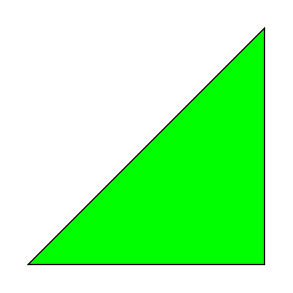
\begin{tikzpicture}
\fill[color=green] (0,0)-- (3,0)--(3,3)--cycle;
\draw[color=black] (0,0)-- (3,0)--(3,3)--cycle;
\end{tikzpicture}

\vskip25pt
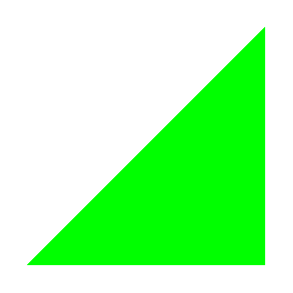
\begin{tikzpicture}
\filldraw[color=green] (0,0)-- (3,0)--(3,3)--cycle;
%\draw[color=black] (0,0)-- (3,0)--(3,3)--cycle;
\end{tikzpicture}

\vskip25pt

\begin{tikzpicture}

\fill[color=yellow] (0,0)rectangle(3,5);
\draw[color=red, line width=4pt] (0,0)rectangle(3,5);
\end{tikzpicture}

\vskip25pt
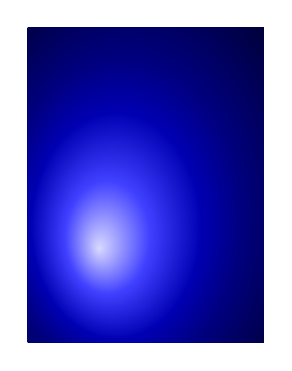
\begin{tikzpicture}
\shade[shading=ball, shading angle=90](0,0) rectangle(3,4);
\end{tikzpicture}

\vskip25pt
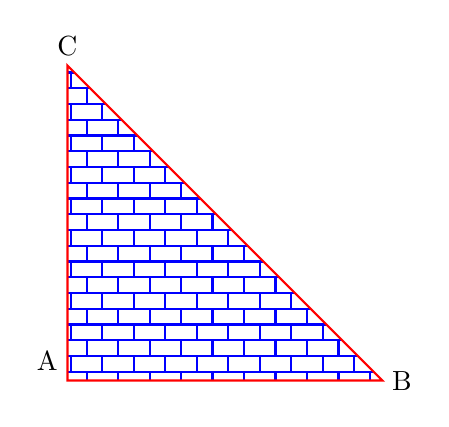
\begin{tikzpicture}
\pattern[pattern=bricks,pattern color=blue](0,0)node[above left]{A}--(4,0)node[right]{B}--(0,4)node[above]{C}--cycle;
\draw[color=red,thick](0,0)--(4,0)--(0,4)--cycle;
\end{tikzpicture}

\begin{tikzpicture}
\path[draw] (0, 0) node[left]{A(0,0)} -- (5,0) -- (5,5) node [above, align=right]{B (5,5)}--cycle;
\end{tikzpicture}
\vskip25pt
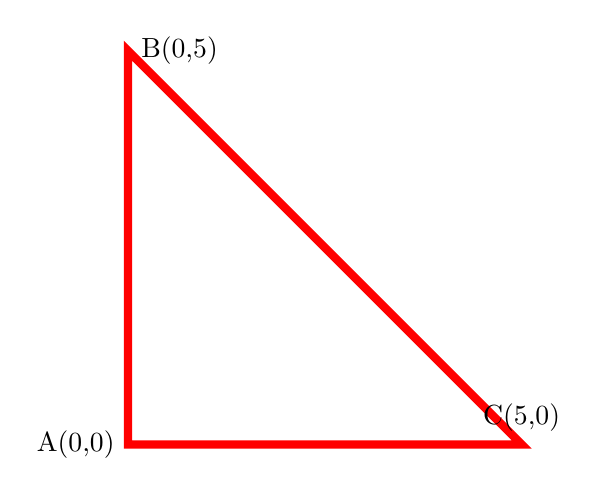
\begin{tikzpicture}
\draw[color=red,line width=3pt](0,0)node[left, align=right,text=black] {A(0,0)}--(0,5)node[right,align=right,text=black] {B(0,5)}--(5,0)node[above,align=right,text=black] {C(5,0)}--cycle;
\end{tikzpicture}
\vskip25pt
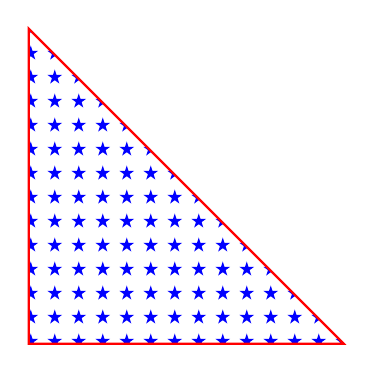
\begin{tikzpicture}
\pattern[pattern=fivepointed stars,pattern color=blue](0,0)--(4,0)--(0,4)--cycle;
\draw[color=red,thick](0,0)--(4,0)--(0,4)--cycle;
\end{tikzpicture}
\vskip35pt
\begin{tikzpicture}
%\fill (0,2) circle (3pt) node[above] {Here!};
\draw (0,0) node[below left] {$A$} --
(4,0) node[below right] {$B$} --
(4,4) node[above right] {$C$} --
(0,4) node[above left] {$D$} -- cycle;
\draw[->](0,0)--(4,0)--(4,4)--(0,4);
\end{tikzpicture}

\vskip30pt
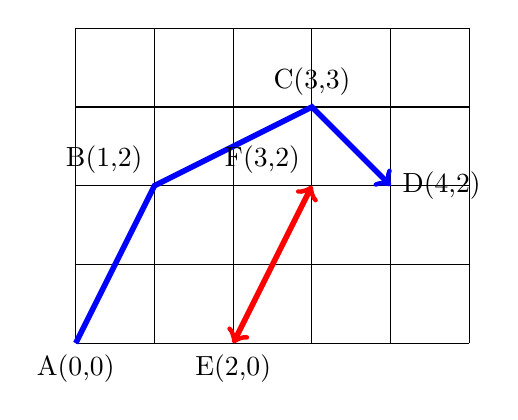
\begin{tikzpicture}
\draw(0,0)grid (5,4);
\draw[->,line width=2,color=blue](0,0)node[below,text=black]{A(0,0)}--(1,2)node[above left,text=black]{B(1,2)}--(3,3)node[above,text=black]{C(3,3)}--(4,2)node[right,text=black]{D(4,2)};
\draw[<->,color=red,line width=2](2,0)node[below,text=black]{E(2,0)}--(3,2)node[above left,text=black]{F(3,2)};
\end{tikzpicture}
\vskip30pt
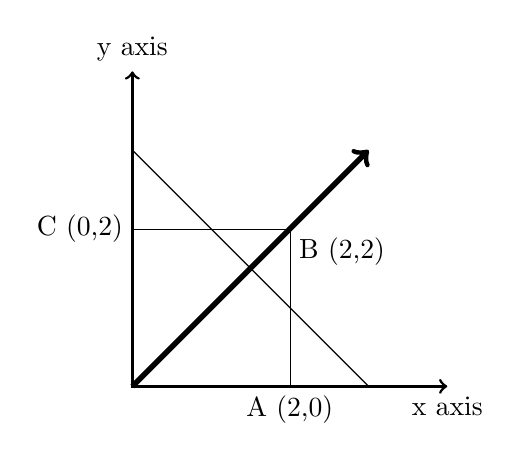
\begin{tikzpicture}
\draw[<->,line width=1](0,4)node[above]{y axis}--(0,0)--(4,0)node[below]{x axis};
\draw[line width=0.5](0,3)--(3,0);
\draw[->, line width=2](0,0)--(3,3);
\draw[line width=0.1](2,0)node[below]{A (2,0)}--(2,2)node[below right]{B (2,2)}--(0,2)node[left]{C (0,2)};
\end{tikzpicture}
\vskip30pt
GRAPH PLOTTING BEGINS HERE
\vskip30pt
\begin{tikzpicture}
%\begin{axis}[xmin=0,xmax=5,ymin=1,ymax=6, xtick distance=1.5,xtick pos=left ]
\begin{axis}[xmin=0,xmax=5,ymin=1,ymax=6,   xtick distance=1,xtick pos=left,ytick pos=left, minor tick num=5 ]
\end{axis}
\end{tikzpicture}




\begin{tikzpicture}
\begin{axis}
\addplot[color=red]{exp(x)};
\end{axis}
\end{tikzpicture}

\begin{tikzpicture}
\begin{axis}
[xmin=-4, xmax=4,ymin=-4,ymax=4, xlabel={x axis label}, ylabel={y axis label}, xlabel style={red,font=\Large,xshift=-7mm}, ylabel style={red, font=\Large, yshift=-3mm}  ]
\end{axis}
\end{tikzpicture}

\begin{tikzpicture}
\begin{axis}
[xmin=-4, xmax=4,ymin=-4,ymax=4, xlabel={x axis label}, ylabel={y axis label}, xlabel style={red,font=\Large,xshift=-7mm}, ylabel style={red, font=\Large, yshift=-2mm}, axis x line=top, axis y line =left  ]
\end{axis}
\end{tikzpicture}


\begin{tikzpicture}
\begin{axis}
[xmin=-4, xmax=4,ymin=-4,ymax=4, xlabel={x axis label}, ylabel={y axis label}, xlabel style={red,font=\Large,xshift=-7mm}, ylabel style={red, font=\Large, yshift=-2mm}, axis x line=bottom, axis y line =left  ]
\end{axis}
\end{tikzpicture}


\begin{tikzpicture}
\begin{axis}
[xmin=-4, xmax=4,ymin=-4,ymax=4, xlabel={x axis label}, ylabel={y axis label}, xlabel style={red,font=\Large,xshift=-7mm}, ylabel style={red, font=\Large, yshift=-2mm}, axis x line=center, axis y line =center  ]
\end{axis}
\end{tikzpicture}

\begin{tikzpicture}
\begin{axis}
[xmin=-4, xmax=4,ymin=-4,ymax=4, xlabel={x axis label}, ylabel={y axis label}, xlabel style={red,font=\Large,xshift=-7mm}, ylabel style={red, font=\Large, yshift=-2mm}, axis x line=bottom, axis y line =middle, title={This is a pfgplots}  ]
\end{axis}
\end{tikzpicture}

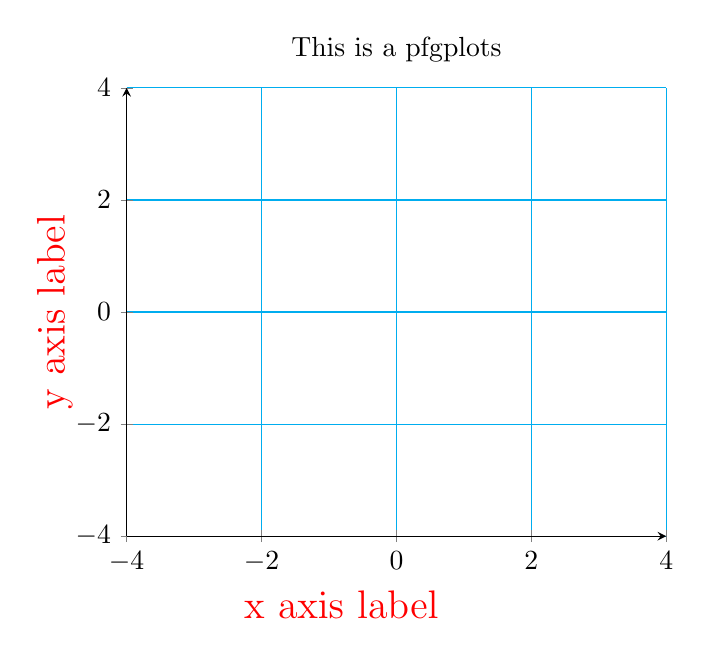
\begin{tikzpicture}
\begin{axis}
[xmin=-4, xmax=4,ymin=-4,ymax=4, xlabel={x axis label}, ylabel={y axis label}, xlabel style={red,font=\Large,xshift=-7mm}, ylabel style={red, font=\Large, yshift=-2mm}, axis x line=bottom, axis y line =left, title={This is a pfgplots}, grid=major, grid style={cyan,opacity=1}  ]
\end{axis}
\end{tikzpicture}

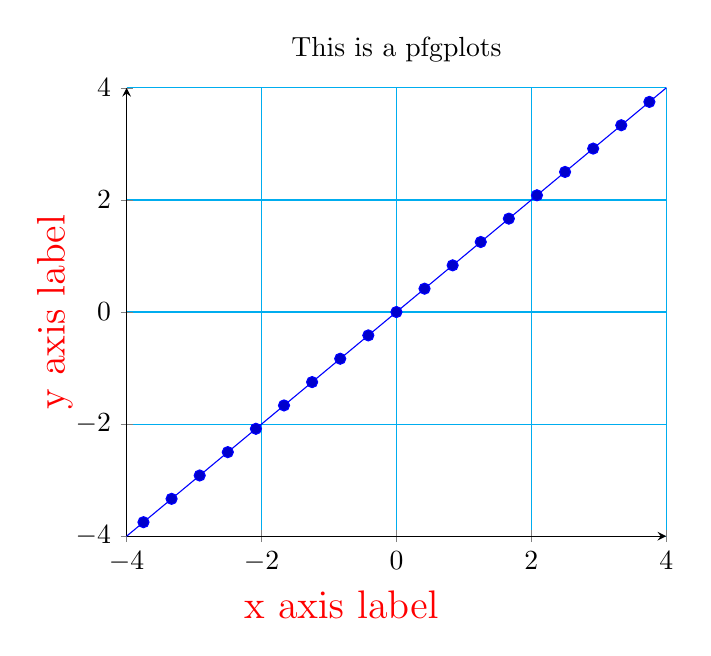
\begin{tikzpicture}
\begin{axis}
[xmin=-4, xmax=4,ymin=-4,ymax=4, xlabel={x axis label}, ylabel={y axis label}, xlabel style={red,font=\Large,xshift=-7mm}, ylabel style={red, font=\Large, yshift=-2mm}, axis x line=bottom, axis y line =left, title={This is a pfgplots}, grid=major, grid style={cyan,opacity=1}  ]
\addplot expression {x};
\end{axis}
\end{tikzpicture}

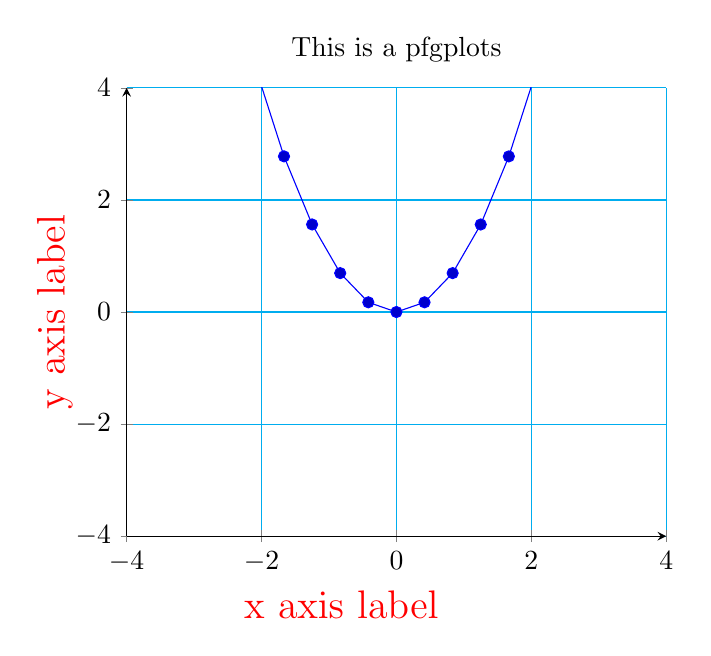
\begin{tikzpicture}
\begin{axis}
[xmin=-4, xmax=4,ymin=-4,ymax=4, xlabel={x axis label}, ylabel={y axis label}, xlabel style={red,font=\Large,xshift=-7mm}, ylabel style={red, font=\Large, yshift=-2mm}, axis x line=bottom, axis y line =left, title={This is a pfgplots}, grid=major, grid style={cyan,opacity=1}  ]
\addplot expression {x^2};
\end{axis}
\end{tikzpicture}

SHIFTINGGGGGGGGGGGGGGGGGGGG axis
sdjfjkdshffjj\\
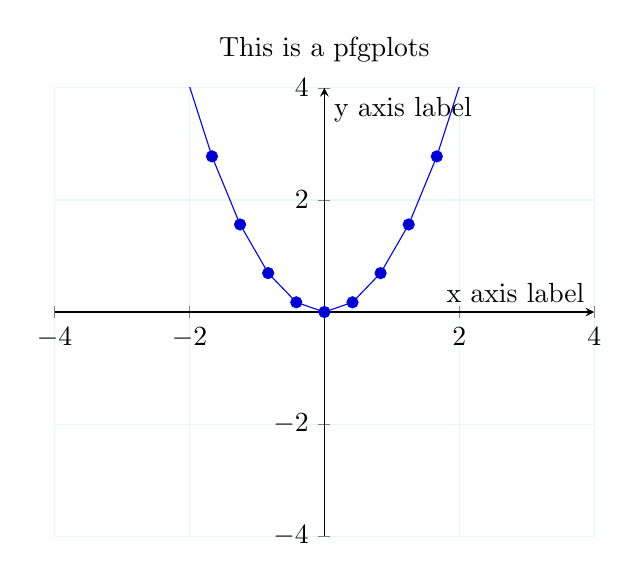
\begin{tikzpicture}
\begin{axis}
[xmin=-4, xmax=4,ymin=-4,ymax=4, xlabel={x axis label}, ylabel={y axis label}, xlabel style={red,font=\Large, xshift=-7mm}, ylabel style={red, font=\Large, yshift=-2mm}, axis x line=middle, axis y line =middle, title={This is a pfgplots}, grid=major, grid style={cyan,opacity=0.1}  ]
\addplot expression {x^2};
\end{axis}
\end{tikzpicture}

\begin{tikzpicture}
\begin{axis}
[xmin=0,xmax=5,ymin=0,ymax=5]
\end{axis}
\end{tikzpicture}


\begin{tikzpicture}
\begin{axis}
[xmin=0,xmax=5,ymin=0,ymax=5, width=7cm,height=7cm]
\end{axis}
\end{tikzpicture}


\begin{tikzpicture}
\begin{axis}
[xmin=0,xmax=5,ymin=0,ymax=5, xtick distance=1.2,ytick distance=1.2]
\end{axis}
\end{tikzpicture}

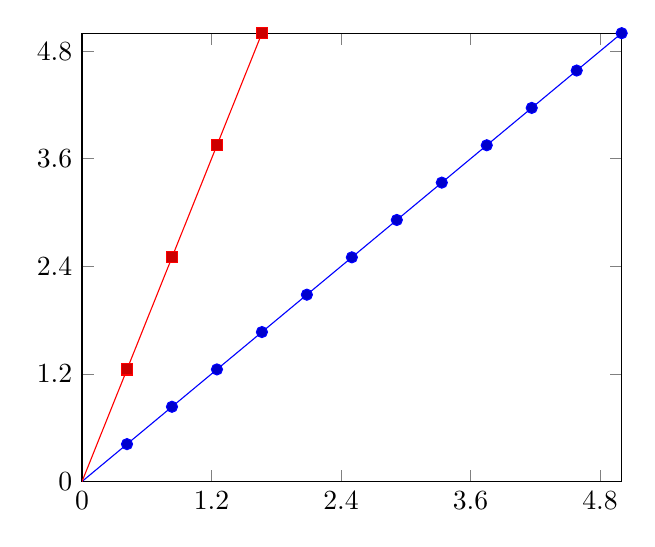
\begin{tikzpicture}
\begin{axis}
[xmin=0,xmax=5,ymin=0,ymax=5, xtick distance=1.2,ytick distance=1.2]
\addplot{x};
\addplot{3*x};
\end{axis}
\end{tikzpicture}

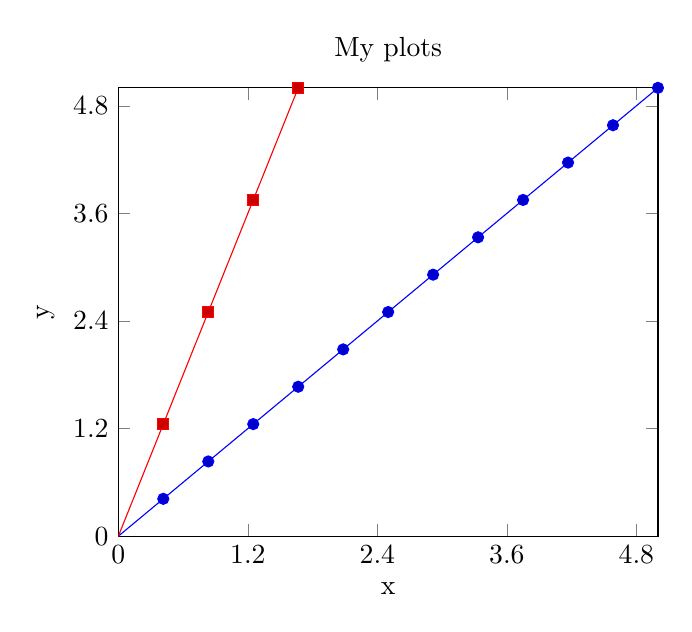
\begin{tikzpicture}
\begin{axis}
[xmin=0,xmax=5,ymin=0,ymax=5, xtick distance=1.2,ytick distance=1.2, xlabel=x,ylabel=y,title={My plots}]
\addplot{x};
\addplot{3*x};
\end{axis}
\end{tikzpicture}


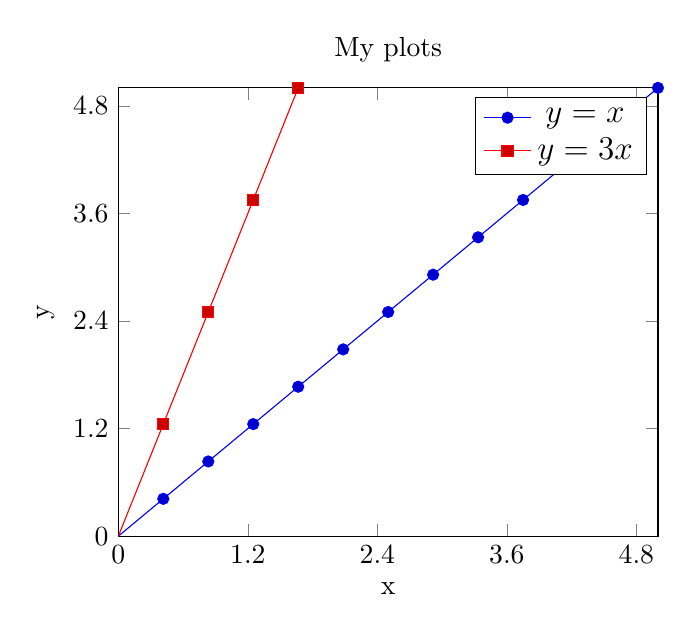
\begin{tikzpicture}
\begin{axis}
[xmin=0,xmax=5,ymin=0,ymax=5, xtick distance=1.2,ytick distance=1.2, xlabel=x,ylabel=y,title={My plots}, legend entries={$y=x$, $y=3x$}, legend style={font=\large}]
\addplot{x};
\addplot{3*x};
\end{axis}
\end{tikzpicture}

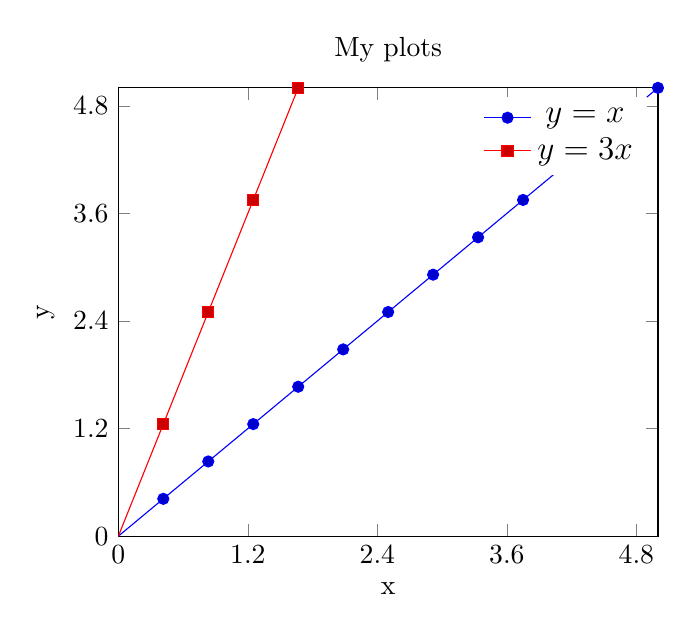
\begin{tikzpicture}
\begin{axis}
[xmin=0,xmax=5,ymin=0,ymax=5, xtick distance=1.2,ytick distance=1.2, xlabel=x,ylabel=y,title={My plots}, legend entries={$y=x$, $y=3x$}, legend style={font=\large,draw=none}]
\addplot{x};
\addplot{3*x};
\end{axis}
\end{tikzpicture}

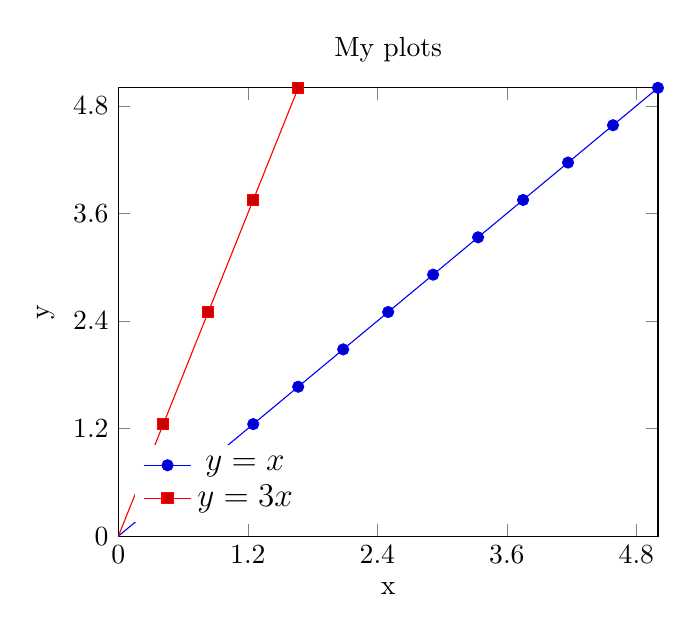
\begin{tikzpicture}
\begin{axis}
[xmin=0,xmax=5,ymin=0,ymax=5, xtick distance=1.2,ytick distance=1.2, xlabel=x,ylabel=y,title={My plots}, legend entries={$y=x$, $y=3x$}, legend style={font=\large,draw=none,legend pos=south west}]
\addplot{x};
\addplot{3*x};
\end{axis}
\end{tikzpicture}

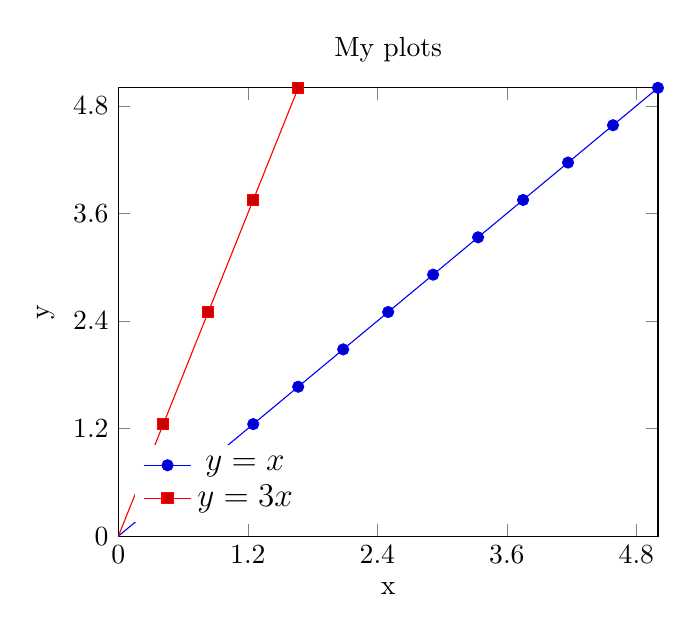
\begin{tikzpicture}
\begin{axis}
[xmin=0,xmax=5,ymin=0,ymax=5, xtick distance=1.2,ytick distance=1.2, xlabel=x,ylabel=y,title={My plots}, legend entries={$y=x$, $y=3x$}, legend style={font=\large,draw=none,legend pos=south west}]
\addplot{x};
\addplot{3*x};
\end{axis}
\end{tikzpicture}


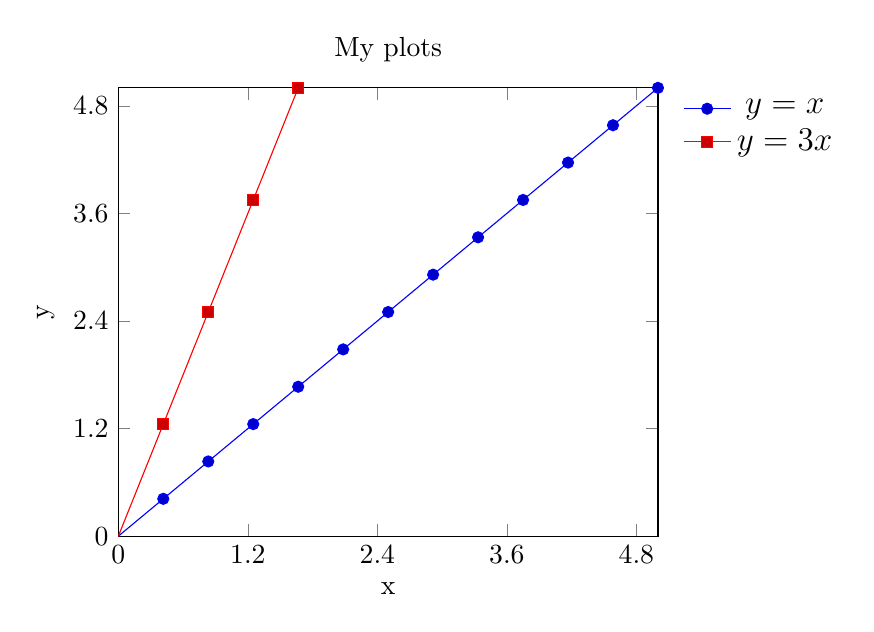
\begin{tikzpicture}
\begin{axis}
[xmin=0,xmax=5,ymin=0,ymax=5, xtick distance=1.2,ytick distance=1.2, xlabel=x,ylabel=y,title={My plots}, legend entries={$y=x$, $y=3x$}, legend style={font=\large,draw=none,legend pos=outer north east}]
\addplot{x};
\addplot{3*x};
\end{axis}
\end{tikzpicture}
\vskip20pt
hereeeeeeeeeeeeeeeeeeeeeeeeeeeeeeeeeeeeeeeee\\

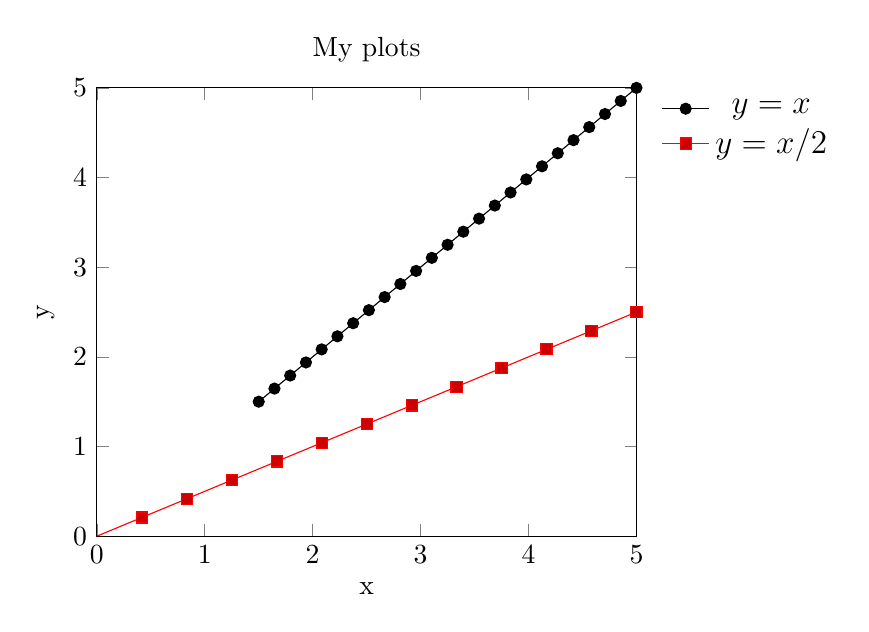
\begin{tikzpicture}
\begin{axis}
[xmin=0,xmax=5,ymin=0,ymax=5,  xlabel=x,ylabel=y,title={My plots}, legend entries={$y=x$, $y=x/2$}, legend style={font=\large,draw=none,legend pos=outer north east}]
\addplot[domain=1.5:5,mark=*]{x};
\addplot{x/2};
\end{axis}
\end{tikzpicture}


\begin{tikzpicture}
\begin{axis}
[xmin=0,xmax=5,ymin=0,ymax=5,  xlabel=x,ylabel=y,title={My plots}, legend entries={$y=x$, $y=x/2$}, legend style={font=\large,draw=none,legend pos=outer north east}]
\addplot[domain=1.5:4.5,mark=*,samples=10]{x};
\addplot[domain=0:5,mark=+,samples=20,red]{x/2};
\end{axis}
\end{tikzpicture}


\begin{tikzpicture}
\begin{axis}
[xmin=0,xmax=5,ymin=0,ymax=5,  xlabel=x,ylabel=y,title={My plots}, legend entries={$y=x$, $y=3x$}, legend style={font=\large,draw=none,legend pos=outer north east}]
\addplot[draw=none,domain=1.5:4.5,mark=*,samples=5]{x};
\addplot[draw=none,domain=0:5,mark=+,samples=20,red]{x/2};
\end{axis}
\end{tikzpicture}

TTTTTTTTTTTTTTTTTTTTTTTTTTTTTTTTTTTTTTTTTTTTTTT
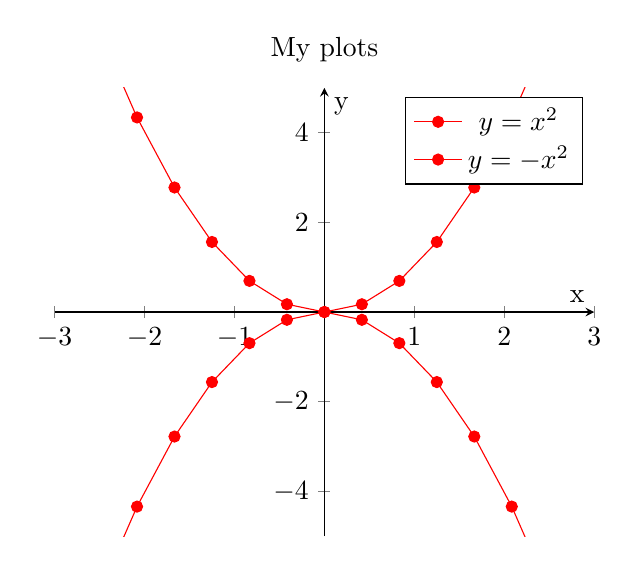
\begin{tikzpicture}
\begin{axis}
[xmin=-3,xmax=3,ymin=-5,ymax=5,  xlabel=x,ylabel=y,title={My plots}, legend entries={$y=x^2$, $y=-x^2$}, axis lines=center]
%\addplot[draw=none,domain=1.5:4.5,mark=*,samples=10]{x};
\addplot[mark=*,red]{x^2};
\addplot[mark=*,red]{-x^2};
\end{axis}
\end{tikzpicture}


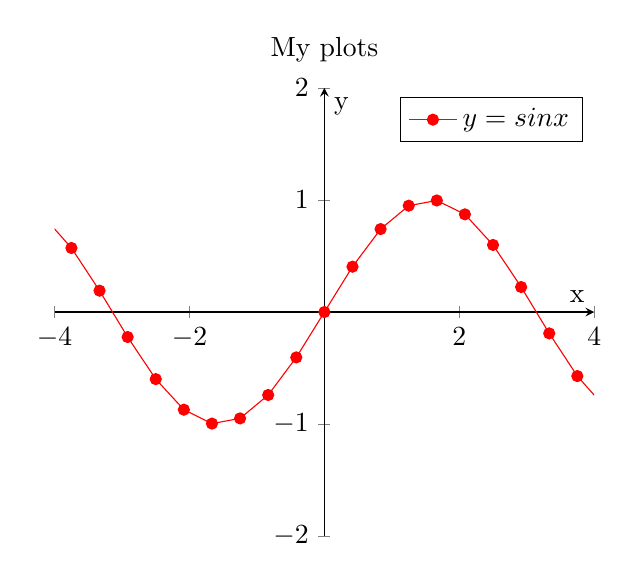
\begin{tikzpicture}
\begin{axis}
[xmin=-4,xmax=4,ymin=-2,ymax=2,  xlabel=x,ylabel=y,title={My plots}, legend entries={$y=sin x$}, axis lines=center]
\addplot[mark=*,red]{sin(deg(x))};
\end{axis}
\end{tikzpicture}












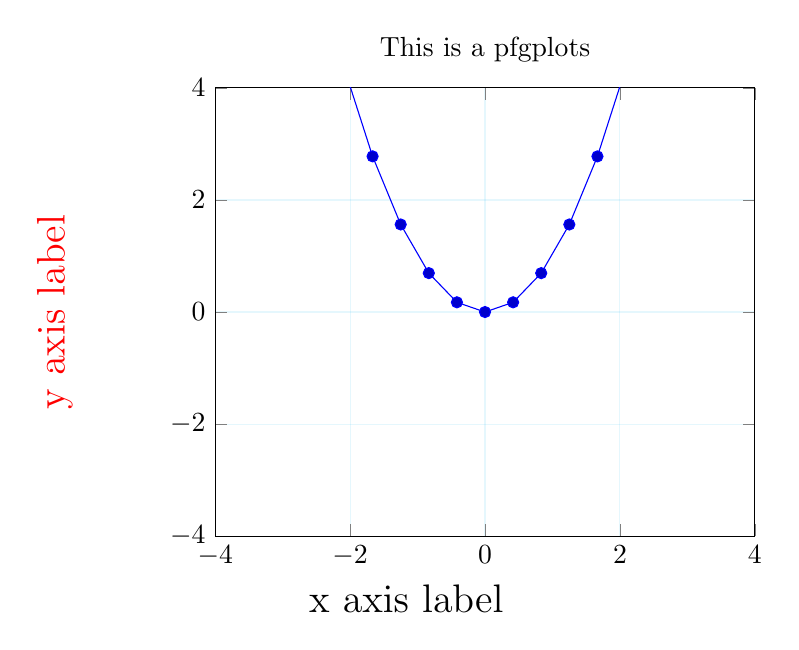
\begin{tikzpicture}
\begin{axis}
[xmin=-4, xmax=4,ymin=-4,ymax=4, xlabel={x axis label}, ylabel={y axis label},
xlabel style={font=\Large, xshift=-10mm}, ylabel style={red, font=\Large, yshift=10mm},  title={This is a pfgplots}, grid=major, grid style={cyan,opacity=0.1}]
\addplot expression {x^2};
\end{axis}
\end{tikzpicture}



\begin{tikzpicture}
\begin{axis}
[xmin=0,xmax=5,ymin=0,ymax=5,  xlabel=x,ylabel=y,title={My plots}, legend entries={$y=x$, $y=x/2$}, legend style={font=\large,draw=none,legend pos=outer north east}]
\addplot[domain=1.5:4.5,mark=*,samples=10]{x};
\addplot[domain=0:5,mark=+,samples=20,red]{x/2};
\end{axis}
\end{tikzpicture}

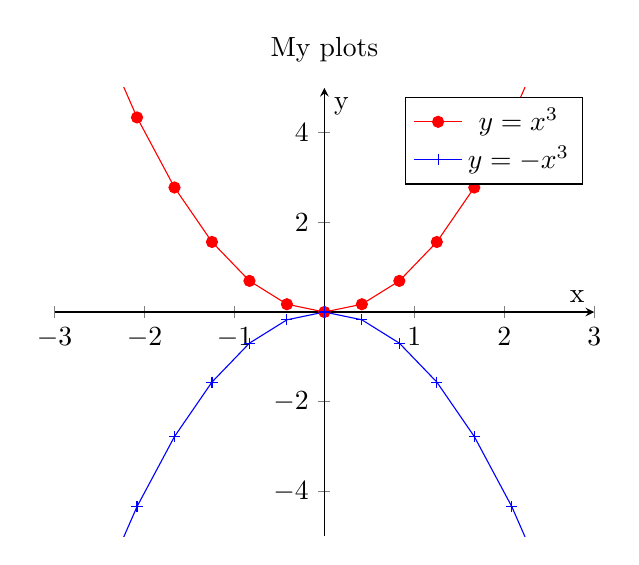
\begin{tikzpicture}
\begin{axis}
[xmin=-3,xmax=3,ymin=-5,ymax=5,  xlabel=x,ylabel=y,title={My plots}, legend entries={$y=x^3$, $y=-x^3$}, axis lines=center]
%\addplot[draw=none,domain=1.5:4.5,mark=*,samples=10]{x};
\addplot[mark=*,red]{x^2};
\addplot[mark=+,blue]{-x^2};
\end{axis}
\end{tikzpicture}

\end{document}
